\documentclass[11pt,oneside,a4paper,fleqn]{memoir}
\usepackage[a4paper,top=4.5cm, bottom=3.5cm, left=2.5cm, right=2.5cm]{geometry}
\usepackage{xcolor}
\usepackage{cite}
\usepackage{amssymb} 
\usepackage{pifont} 
\usepackage{rotating}
\usepackage{graphicx}
\usepackage{url}
\usepackage{mathtools}
\usepackage{amsmath}
\usepackage{mathtools}
\setlength{\mathindent}{0pt}
%drawing libraries
\usepackage{tikz}
\usetikzlibrary{shapes}
% Optional PGF libraries
\usepackage{pgflibraryarrows}
\usepackage{pgflibrarysnakes}

\newcommand{\cmark}{\ding{51}}%
\newcommand{\xmark}{\ding{55}}%

\begin{document}
\pagecolor{white}
%left bottom right top
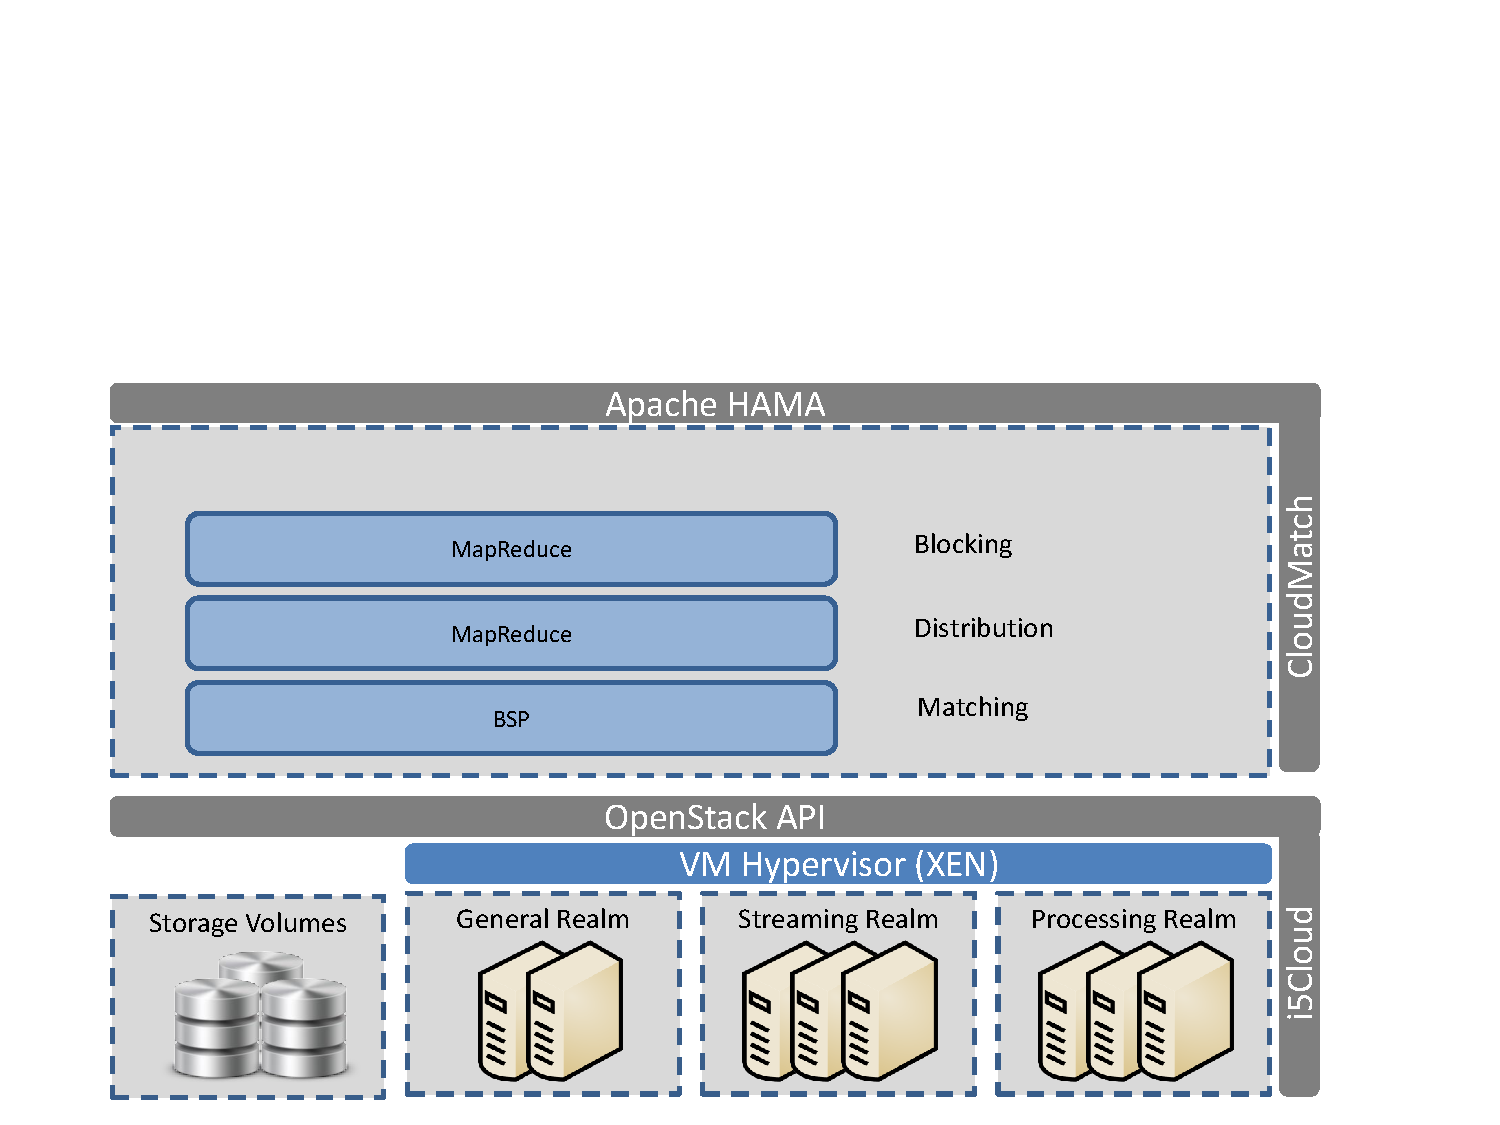
\includegraphics[page=1,trim = 15mm 0mm 30mm 60mm, clip,scale=0.5]{Architecture_block_diagram_Detailed}  

i5Cloud is cloud computing platform hosted by the data and information systems chair in RWTH Aachen. the first version i5Cloud 0.1 used Sun Enterprise server with Sun SPARC T5240 architecture. The current version i5Cloud 0.2 uses Sun server with Sun Fire x4450 architecture. This server system can expand to up to 24 processing cores, 256 GB of memory, and more than 2 TB of internal storage. i5Cloud 0.2 hosts the OpenStack\footnote{\url{http://www.openstack.org/}} open-source project for cloud infrastructure management.
\end{document}
\section{i5Cloud}
